% arara: pdflatex: { synctex: yes }
% arara: makeindex: { style: ctuthesis }
% arara: bibtex

% The class takes all the key=value arguments that \ctusetup does,
% and a couple more: draft and oneside
\documentclass[twoside]{ctuthesis}

\ctusetup{
	preprint = \ctuverlog,
	mainlanguage = english,
	titlelanguage = english,
%	mainlanguage = czech,
	otherlanguages = {slovak,english},
	title-czech = {Moje bakalářka se strašně, ale hrozně dlouhým předlouhým názvem},
	title-english = {Drone detection using neural networks from combined RGB camera and LiDAR data},
	subtitle-czech = {Cesta do tajů kdovíčeho},
%	subtitle-english = {Journey to the who-knows-what wondeland},
	doctype = B,
	faculty = F3,
	department-czech = {Katedra matematiky},
	department-english = {Department of Cybernetics},
	author = {Adam Škuta},
	supervisor = {Matouš Vrba},
	supervisor-address = {Ústav X, \\ Uliční 5, \\ Praha 99},
	supervisor-specialist = {Martin Saska},
	fieldofstudy-english = {Mathematical Engineering},
	subfieldofstudy-english = {Mathematical Modelling},
	fieldofstudy-czech = {Matematcké inženýrství},
	subfieldofstudy-czech = {Matematické modelování},
	keywords-czech = {slovo, klíč},
	keywords-english = {word, key},
	day = 10,
	month = 2,
	year = 2017,
	specification-file = {ctutest-zadani.pdf},
%	front-specification = true,
%	front-list-of-figures = false,
%	front-list-of-tables = false,
%	monochrome = true,
%	layout-short = true,
}

\ctuprocess

\addto\ctucaptionsczech{%
	\def\supervisorname{Vedoucí}%
	\def\subfieldofstudyname{Studijní program}%
}

\ctutemplateset{maketitle twocolumn default}{
	\begin{twocolumnfrontmatterpage}
		\ctutemplate{twocolumn.thanks}
		\ctutemplate{twocolumn.declaration}
		\ctutemplate{twocolumn.abstract.in.titlelanguage}
		\ctutemplate{twocolumn.abstract.in.secondlanguage}
		\ctutemplate{twocolumn.tableofcontents}
		\ctutemplate{twocolumn.listoffigures}
	\end{twocolumnfrontmatterpage}
}

% Theorem declarations, this is the reasonable default, anybody can do what they wish.
% If you prefer theorems in italics rather than slanted, use \theoremstyle{plainit}
\theoremstyle{plain}
\newtheorem{theorem}{Theorem}[chapter]
\newtheorem{corollary}[theorem]{Corollary}
\newtheorem{lemma}[theorem]{Lemma}
\newtheorem{proposition}[theorem]{Proposition}

\theoremstyle{definition}
\newtheorem{definition}[theorem]{Definition}
\newtheorem{example}[theorem]{Example}
\newtheorem{conjecture}[theorem]{Conjecture}

\theoremstyle{note}
\newtheorem*{remark*}{Remark}
\newtheorem{remark}[theorem]{Remark}

\setlength{\parskip}{5ex plus 0.2ex minus 0.2ex}
\graphicspath{{figures/}}

% Abstract in Czech
\begin{abstract-czech}
\end{abstract-czech}

% Abstract in English
\begin{abstract-english}
\end{abstract-english}

% Acknowledgements / Podekovani
\begin{thanks}
Děkuji ČVUT, že mi je tak dobrou \emph{alma mater}.
\end{thanks}

% Declaration / Prohlaseni
\begin{declaration}
Prohlašuji, že jsem předloženou práci vypracoval samostatně, a že jsem uvedl veškerou použitou literaturu.

V Praze, \ctufield{day}.~\monthinlanguage{title}~\ctufield{year}
\end{declaration}

% Only for testing purposes
\listfiles
\usepackage[pagewise]{lineno}
\usepackage{lipsum,blindtext}
\usepackage{mathrsfs} % provides \mathscr used in the ridiculous examples
\usepackage{todonotes}
\usepackage{amsmath}
\usepackage{xspace}

\begin{document}

\maketitle
\chapter{Introduction}
The goal of this thesis is to prove whether a usage of LiDAR data coupled with images from RGB is useful for the localization of UAVs in contrast to the usage of image data alone. The LiDAR and RGB camera will be mounted on top of the scanner UAV. All the measurements will be taken inside a virtual environment, with a realistic UAV and sensor simulation. The dataset will then be preprocessed and used as the input to a Convolutional neural network for the object detection. The preprocessing will be as following:
\begin{itemize}
	\item Coordinate transformation for the non-matching coordinate systems
	\item Projection of 3d points into a 2d image
	\item Using a Convolutional neural network to generate more points in a sparse LiDAR pointcloud
\end{itemize}
\todo{Infographic of the process}
\chapter{Convolutional neural networks}
A convolutional neural network will be used in two problems in the thesis. First one is used on a sparse LiDAR pointcloud generating more points and therefore making it more dense. Second one is used for object, int this case drone, detection, using RGB and RGBD data as the input.
\section{Sparse to dense}
Sparse to dense is a Convolutional neural network written in PyTorch. It predicts the depth measurements from sparse depth dataset. The size of the network is modifiable and can be chosen as training parameters.
\begin{figure}[h!]
	\caption{Example of different network architectures available}
	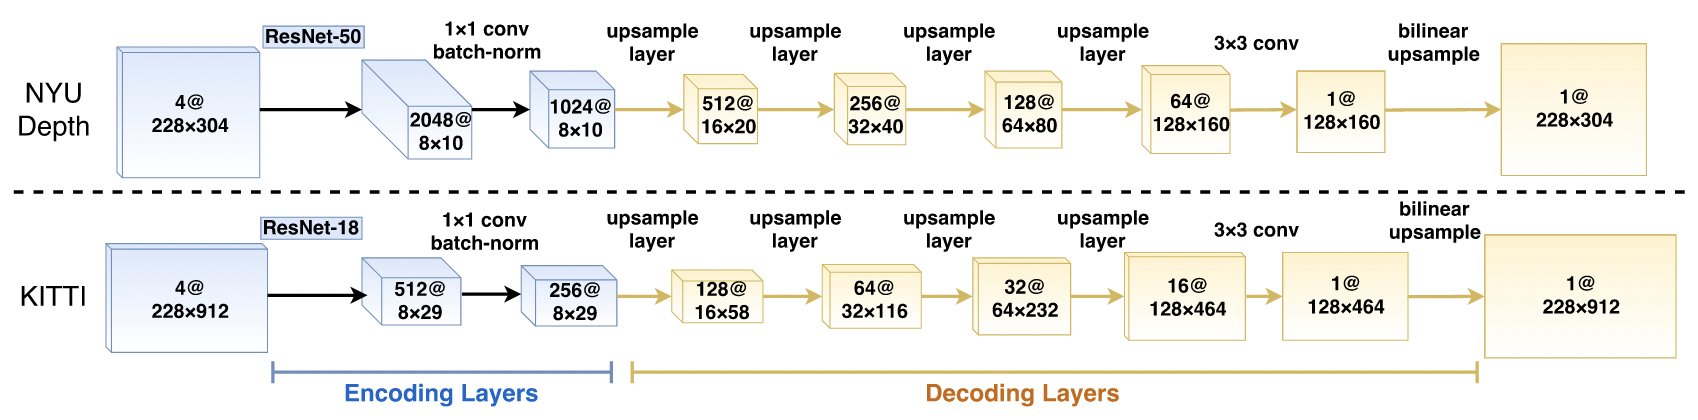
\includegraphics[width=\textwidth]{sparse2dense.png}
	\centering
\end{figure}\\
For the encoding and therefore input layers a ResNet-50 or ResNet-18 can be chosen, depending on the size of the input image for memory constraints. The decoding layers consist of 4 upsampling layers and a deconvolutional layer with either stride 2 or 3 or uprojection layer or upconvolutional layer as a choice for training. The default loss function is least absolute deviations also known as $L_1$ error:
\begin{equation}
	L_1=\sum_{i=1}^{n}|y_{true}-y_{predicted}|
\end{equation}
where:
\begin{itemize}
	\item n is batch size
	\item $y_{true}$ are real depth values
	\item $y_{predicted}$ are predicted depth values
\end{itemize}
The input to the network are RGBD images and the output is a depth map with the same dimensions as input. The depth input $D$ is sampled from the ground truth depth map $D^*$ with the following formula:
\begin{equation}
	D(i,j)=\begin{cases}
		D^*(i,j),&\text{with probability}\ p\\
		0,&\text{otherwise}
	\end{cases}
\end{equation}
where:
\begin{itemize}
	\item $i,j$ are coordinates of the input image
	\item $p=\frac{m}{n}$, where $m$ number of depth samples to be chosen at the start of training and $n$ is the total amount of available depth samples
\end{itemize}
During training several input data augmentations take place. These augmentations include:
\begin{itemize}
	\item Scaling the input image by a random number $s\in[1,1.5]$
	\item Rotating the input image by a random degree $r\in[-5,5]$
	\item Scaling the brightness, contrast and saturation of the RGB component of the image by a random number $k\in[0.6,1.4]$
	\item Normalizing the RGB component of the image
	\item Flipping the image horizontally with a 50\% chance
\end{itemize}
The output of the network is a dense depth image with the dimensions of the input. Every pixel contains predicted depth measurement in meters. The output of the Sparse to Dense network will be used for further training later.
\section{YOLOv3}
\todo{citations}
You only look once (YOLO) is a convolutional neural network model used mainly for object detection and recognition. The main advantage is its simplicity in comparison to similar convolutional neural networks, resulting in faster detection speeds. It belongs to the state of the art convolutional neural networks for object detection and recognition. The version used in this work is the third version YOLOv3. The backbone called Darknet53 consists of 53 convolutional layers. The original detector consists of 3 detection heads each responsible for detecting objects of various sizes.
\begin{figure}[h]
	\caption{YOLOv3 network architecture}
	\centering
	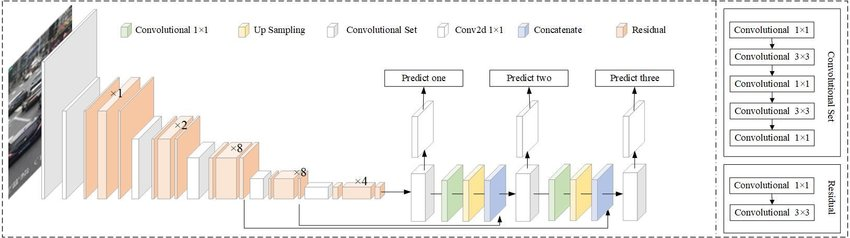
\includegraphics[width=\textwidth]{yolov3model.jpg}
\end{figure}
YOLOv3 takes $n$-channel images as the input and outputs are as following:
\begin{itemize}
	\item Offsets of the bounding box centers relative to the size of input image
	\item Scales of the bounding boxes relative to their respective anchors
	\item Objectness score, which dictates the confidence of object detection in the particular cell
	\item Class score, which dictates the confidence of object recognition in the particular cell for each of the classes used during training
\end{itemize}
The loss function used during the training was sum squared error loss or $L_2$ error described as follows:
\begin{equation}
	L_2=\sum_{i=1}^{n}(y_{true}-y_{predicted})^2
\end{equation}
where:
\begin{itemize}
	\item $n$ is batch size
	\item $y_{true}$ are ground truth bounding box values
	\item $y_{predicted}$ are predicted bounding box values
\end{itemize}

\chapter{Sensors}
\section{Coordinate systems}
In order to correctly label the data for training, a position of the second drone in relation to the camera mounted on the first one is required. The API call in AirSim returns a position in relation to its starting point.\todo{insert picture showing the positions of the drones} Therefore a transformation from the starting point of the second drone to the camera mounted on the first one is required. We can write this transformation as follows:
\begin{equation}
	\textbf{T}=\textbf{T}_{d1}^{c}\textbf{T}_{s1}^{d1}\textbf{T}_{s2}^{s1}
\end{equation}
where:
\begin{itemize}
	\item $\textbf{T}_{s2}^{s1}$ is transformation from the starting point of the second drone to the starting point of the first drone
	\item $\textbf{T}_{s1}^{d1}$ is transformation from the starting point of the first drone to the body of the first drone
	\item $\textbf{T}_{d1}^{c}$ is transformation from the body of the first drone to the cameras coordinate system
\end{itemize}
Transformation matrix $\textbf{T}$ can generally be described as follows:
\begin{equation}
	\textbf{T}=\begin{bmatrix}
		\textbf{R} & \textbf{p}\\
		\textbf{0}^T & 1
	\end{bmatrix}
\end{equation}
where:
\begin{itemize}
	\item $\textbf{R}$ is a 3x3 rotation matrix
	\item $\textbf{p}$ is a 3x1 translation column vector
	\item $\textbf{0}^T$ is a 1x3 row vector of zeros
\end{itemize}
\section{Camera Model}
For the creation of the bounding boxes used for training a transformation from coordinate system of the camera to the pixel values of the image needs to be defined. For this task a pinhole camera model is used.\todo{Picture of pinhole camera}
The transformation is then defined as follows:
\begin{equation}
	\begin{bmatrix}
		x'\\
		y'
	\end{bmatrix}=
	\begin{bmatrix}
		f\frac{x}{z}+c_x\\
		f\frac{y}{z}+c_y
	\end{bmatrix}
\end{equation}
where:
\begin{itemize}
	\item $x'$ and $y'$ are pixel coordinate values on the image
	\item $x$,$y$,$z$ are coordinate values of a point to be transformed
	\item $f$ is focal length of the camera
	\item $c_x$,$c_y$ are offsets on the image plane
\end{itemize}
\chapter{Dataset}
The dataset for this work can be generated in two ways. The first is real-life drone shots mixed with point clouds from LiDAR mounted on top of a drone. The second is generating a dataset using a realistic virtual environment where a drone, camera and LiDAR are being emulated very close to their real-life counterparts. An advantage to this approach is that a great variety of environments can be chosen a lot of them often inaccessible otherwise (power plant, airport, snowy mountains out of season etc.). Therefore this approach will be chosen for the task.
\section{Unreal Engine}
Unreal Engine is a software tool used for creating realistic 3d environments, most often used as a video game engine.
\todo{citation https://www.unrealengine.com/en-US/features} 
It is written in C++ and open-source supporting a variety of pre-built environments and assets. For this work three diferent environments will be used for the creation of the dataset:
\begin{itemize}
	\item \todo[inline]{exact name. Snow}
	\item \todo[inline]{exact name. Park}
	\item \todo[inline]{exact name. City centre}
\end{itemize}
\todo{Pictures of the environments}
Together \todo[inline]{exact number of pictures} pictures and labels were generated using two drones. One drone was equipped with RGB camera and LiDAR sensor and was responsible for taking the pictures and pointclouds from LiDAR. The second one was used as a model for drone detection.
\section{AirSim}
Open-source plugin for Unreal Engine called AirSim was used for the generation of the dataset. It simulates realistic flight motions of drones as well as seven types of sensors \todo{airsim zdroj}, including RGB camera and LiDAR used for this task. AirSim supports both a C++ API as well as Python API, latter which was used for controlling the motion and capturing the dataset. Location of the second drone was generated through API call, which produces a location of the drone in global coordinate system of the map, which is later transformed to the local coordinates of the first drone carrying the LiDAR and RGB sensors.\todo{Transformacna matica?}. The capturing drone traveled on each map on a 3d cube grid:\todo[inline]{Grafika kocky po ktorej lietal dron}
\chapter{Training}
For the training purposes 5320 samples were taken using AirSim simulator. Each sample consists of:
\begin{itemize}
	\item 640x640 3-channel RGB image from the camera
	\item 640x640 1-channel sparse depth image from the LiDAR sensor
	\item Label file containing ground truth bounding boxes values
\end{itemize}
This dataset was split 90\% training samples to 10\% validation samples. 
\section{Sparse to Dense}
First the data were trained using Sparse to Dense neural network to receive dense depth image. The training was done for 15 epochs using batch size of 8. The backbone was Resnet18 and decoder was set to Deconv3. The network was pretrained on Kitti dataset. \todo{put images of the sparse2dense output}
\section{Preprocessing}
After the first network trained multiple methods of preprocessing were used.
\end{document}
